\chapter{Goniometria}
\section{Angoli}
\begin{figure} %[htbp]
	\centering
	\includestandalone[width=.6\textwidth]{funzgonioTikz/angoliconcaviconvessi}
	\caption{Angoli concavi e convessi, positivi e negativi}
	\label{fig:angconconvposoneg}
	\end{figure}
	\begin{figure} %[htbp]
		\centering
		\includestandalone[width=\textwidth]{funzgonioTikz/angolinotevoli}
		\caption{Angoli notevoli}
		\label{fig:Angolorettoposneggonio}
		\end{figure}
		\begin{figure}
			\includestandalone[width=\textwidth]{funzgonioTikz/mappagomiometricaangolo}
			\caption{Mappa goniometria l'angolo}
			\label{fig:MappaGonometria1}
		\end{figure}
\section{Radianti}
\begin{figure}
	\centering
	\includestandalone[width=7.5cm]{funzgonioTikz/radianti}
	\caption{Radianti}
	\label{fig:radinatidefgonio}
\end{figure}
\section{Circonferenza goniometrica}
\begin{figure}
	\centering
	\includestandalone[width=7.5cm]{funzgonioTikz/circonferenzagoniometrica}
	\captionof{figure}{Circonferenza goniometrica}
	\label{fig:circonferenzagonimetricagonio}
\end{figure}
\begin{figure}
	\centering
	\includestandalone[width=20cm]{funzgonioTikz/CirGonioSpecial}
	\captionof{figure}{Circonferenza goniometrica}
	\label{fig:circonferenzagonimetricagonio2}
\end{figure}
\begin{figure}
	\begin{subfigure}[b]{.5\linewidth}
		\centering
		\includestandalone[width=5cm]{funzgonioTikz/cosenodefinizione}
		\caption{Coseno definizione}\label{sub:cosenodef}
	\end{subfigure}%
	\begin{subfigure}[b]{.5\linewidth}
		\centering
		\includestandalone[width=7.5cm]{funzgonioTikz/cosenografico}
		\caption{Coseno grafico}\label{sub:cosenograf}
	\end{subfigure}
	\captionof{figure}{Coseno}
	\label{tab:funzcos}
\end{figure}
\begin{figure}
	\begin{subfigure}[b]{.5\linewidth}
		%		\centering\includegraphics[scale=0.35]{senoalpha-crop}
		\centering
		\includestandalone[width=5cm]{funzgonioTikz/senodefinizione}
		\caption{Seno definizione}\label{sub:senodef}
	\end{subfigure}%
	\begin{subfigure}[b]{.5\linewidth}
		\centering
		\includestandalone[width=7.5cm]{funzgonioTikz/senografico}
		\caption{Seno grafico}\label{sub:senograf}
	\end{subfigure}
	\captionof{figure}{Seno}
	\label{tab:funseno}
\end{figure}
\begin{figure}
	\centering
	\includestandalone[width=8.5cm]{funzgonioTikz/andamentoseno1}
	\captionof{figure}{Andamento seno $\ang{0}<\alpha<\ang{180}$}\label{fig:AndamentoSeno1}
\end{figure}%
\begin{figure}
	\centering
	\includestandalone[width=8.5cm]{funzgonioTikz/andamentoseno2}
	\captionof{figure}{Andamento seno $\ang{180}<\alpha<\ang{360}$}\label{fig:AndamentoSeno2}
\end{figure}%
\begin{figure}
	\begin{subfigure}[b]{.5\linewidth}
		\centering\includestandalone[width=0.6\textwidth]{funzgonioTikz/segnocoseno}
		\caption{Segno coseno}\label{fig:SegnoCoseno}
	\end{subfigure}%
	\begin{subfigure}[b]{.5\linewidth}
		\centering\includestandalone[width=0.6\textwidth]{funzgonioTikz/segnoseno}
		\caption{Segno seno}\label{fig:SegnoSeno}
	\end{subfigure}
	\begin{subfigure}[b]{.5\linewidth}
		\centering\includestandalone[width=0.6\textwidth]{funzgonioTikz/segnotangente}
		\caption{Segno tangente}\label{fig:SegnoTangente}
	\end{subfigure}%
	\begin{subfigure}[b]{.5\linewidth}
		\centering\includestandalone[width=0.6\textwidth]{funzgonioTikz/segnocotangente}
		\caption{Segno cotangente}\label{fig:SegnoCotangente}
	\end{subfigure}
	\captionof{figure}{Segno funzioni goniometriche}
	\label{tab:segnofunzionigoniometriche}
\end{figure}
\begin{figure}
	\begin{subfigure}[b]{.5\linewidth}
		\centering
		\includestandalone[width=5cm]{funzgonioTikz/tangentedefinizione}
		\caption{Tangente definizione}\label{fig:TangenteDefinizione}
	\end{subfigure}%
	\begin{subfigure}[b]{.5\linewidth}
		\centering\includestandalone[width=7.5cm]{funzgonioTikz/tangentegrafico}
		\caption{Tangente grafico}\label{fig:TangenteGrafico}
	\end{subfigure}
	\captionof{figure}{Tangente}
	\label{tab:funztg}
\end{figure}
\begin{figure}
	\centering
	\includestandalone[width=8.5cm]{funzgonioTikz/tangenteandamento1}
	\captionof{figure}{Andamento tangente $\ang{0}<\alpha<\ang{180}$}\label{fig:AndamentoTangente1}
\end{figure}%
\begin{figure}
	\centering
	\includestandalone[width=8.5cm]{funzgonioTikz/tangenteandamento2}
	\captionof{figure}{Andamento tangente $\ang{180}<\alpha<\ang{360}$}\label{fig:AndamentoTangente2}
\end{figure}%
\begin{figure}
	\begin{subfigure}[b]{.5\linewidth}
		\centering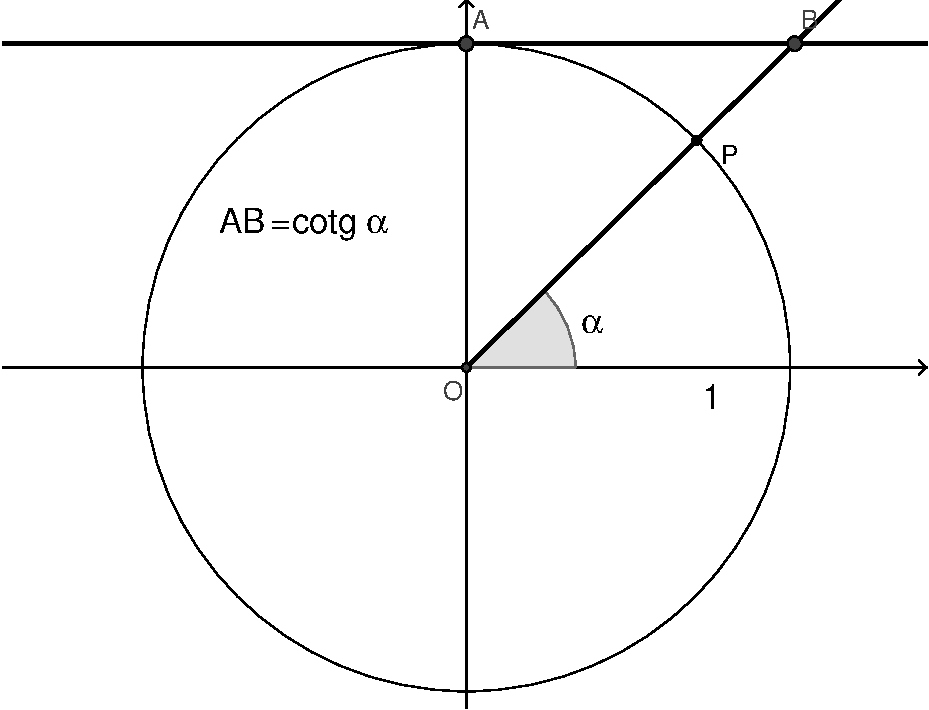
\includegraphics[scale=0.3]{cotgalpha-crop}
		\caption{Cotangente}\label{fig:CotangenteDefinizione}
	\end{subfigure}%
	\begin{subfigure}[b]{.5\linewidth}
		\centering\includegraphics[scale=0.3]{cotgalphagrafico-crop}
		\caption{Cotangente grafico}\label{fig:CotangenteGrafico}
	\end{subfigure}
	\captionof{figure}{Cotangente}
	\label{tab:funzcotg}
\end{figure}
\begin{figure}
	\centering
	\includestandalone[width=8.5cm]{funzgonioTikz/cotangenteandamento1}
	\captionof{figure}{Andamento cotangente $\ang{0}<\alpha<\ang{180}$}\label{fig:AndamentoCotangente1}
\end{figure}%
\begin{figure}
	\centering
	\includestandalone[width=8.5cm]{funzgonioTikz/cotangenteandamento2}
	\captionof{figure}{Andamento cotangente $\ang{180}<\alpha<\ang{360}$}\label{fig:AndamentoCotangente2}
\end{figure}%
\begin{figure}
	\centering
	\begin{tikzpicture}[>=triangle  45]
	% draw the coordinates
	
	\pgfmathsetmacro{\raggio}{4};
	\pgfmathsetmacro{\mraggio}{\raggio/6};
	
	\pgfmathsetmacro{\sraggio}{1.9*\raggio};
	\draw[->] (0,-\raggio/2-\mraggio/2) -- (0,\raggio+\mraggio) node[above,fill=white] {$y$};
	\draw[->] (-\raggio/2-\mraggio/2,0) -- (\raggio+\mraggio,0) node[right,fill=white] {$x$};
	\node(OO)at(0,0) [label= above left:$O$] {};
	\foreach \x/ \y/\arco  in {
		55/5/{\alpha}%,
	}
	{
		\draw[->] (\sraggio/\y,0 ) arc (0:\x:\sraggio/\y);% node[above ] {$\arco$};
		\node (aa) at   ({cos(\x/2} , {sin(\x/2} ) [label=above:$\arco$] {};
		\draw(0,0) -- ({\raggio*cos(\x} , {\raggio*sin(\x})node[midway ]{a} node [above]{P};
		\draw[dashed] ({\raggio*cos(\x} , 0 ) -- ({\raggio*cos(\x} , {\raggio*sin(\x} )node[midway ]{c}  ;
		\draw [dashed](0, {\raggio*sin(\x} ) -- ({\raggio*cos(\x} , {\raggio*sin(\x} );
		\draw[dashed] (0 , 0 ) -- (0 , {\raggio*sin(\x} )node [above]{K};
		\draw [dashed](0, 0 ) -- ({\raggio*cos(\x} , 0 )node[midway ]{b} node [above]{H};;
	}
	\draw plot[domain=0:90,smooth] ({\raggio*cos(\x} , {\raggio*sin(\x});
	\end{tikzpicture}
	\caption{Relazione fondamentale goniometria}
	\label{fig:relFondGonio}
\end{figure}
\begin{figure}
	\begin{subfigure}[b]{.5\linewidth}
		\caption{}\centering\includestandalone[width=0.6\textwidth]{funzgonioTikz/CosenoNotoSeno1}
		\caption{}\label{fig:CosenoNotoSeno1}
	\end{subfigure}%
	\begin{subfigure}[b]{.5\linewidth}
		\centering\includestandalone[width=0.6\textwidth]{funzgonioTikz/CosenoNotoSeno2}
		\caption{}\label{fig:CosenoNotoSeno2}
	\end{subfigure}
	\begin{subfigure}[b]{.5\linewidth}
		\centering\includestandalone[width=0.6\textwidth]{funzgonioTikz/CosenoNotoSeno3}
		\caption{}\label{fig:CosenoNotoSeno3}
	\end{subfigure}%
	\begin{subfigure}[b]{.5\linewidth}
		\centering\includestandalone[width=0.6\textwidth]{funzgonioTikz/CosenoNotoSeno4}
		\caption{}\label{fig:CosenoNotoSeno4}
	\end{subfigure}
	\captionof{figure}{Coseno noto seno}
	\label{fig:CosenoNotoSenoEs1}
\end{figure}
\begin{figure}
	\begin{subfigure}[b]{.5\linewidth}
		\caption{}\centering\includestandalone[width=0.6\textwidth]{funzgonioTikz/senoNotoCoseno1}
		
		\caption{}\label{fig:senoNotoCoseno1}
	\end{subfigure}%
	\begin{subfigure}[b]{.5\linewidth}
		\centering\includestandalone[width=0.6\textwidth]{funzgonioTikz/senoNotoCoseno2}
		\caption{}\label{fig:senoNotoCoseno2}
	\end{subfigure}
	\begin{subfigure}[b]{.5\linewidth}
		\centering\includestandalone[width=0.6\textwidth]{funzgonioTikz/senoNotoCoseno3}
		\caption{}\label{fig:senoNotoCoseno3}
	\end{subfigure}%
	\begin{subfigure}[b]{.5\linewidth}
		\centering\includestandalone[width=0.6\textwidth]{funzgonioTikz/senoNotoCoseno4}
		\caption{}\label{fig:senoNotoCoseno4}
	\end{subfigure}
	\captionof{figure}{Seno Noto Coseno}
	\label{fig:senoNotoCosenoEs1}
\end{figure}